% Admir, Anna,  Sune (prototype)

% API implementation - Google, Firebase, Activity Recognition (Admir)
% Data Collection - Geofence, Activity Recognition, Location (Sune) - blir det ikke forklaret i subsection 5.2
% Search (Sune)
% Distance calculator
% ILocation and IStorage or other with interface and listener
% Adapter view pattern (Anna)

% TODO:
% Apply definitions
% Introduction
% Explain three different categories of prototyping
%    - Explorative, Experimental, Evoulutionary


In the following sections, central aspects of the BikeBus solution will be highlighted. This are applied examples on compression techniques and examples of architectural designs. Several different Google services are also touched upon, including the data layer implementation.

% TODO:
% Explain all protoypes in our program (Implementation)
%    - Datastructures, algorithms, storage, etc
%    - Diagrams
%    - Results of prototypes

% Current Prototypes:
% - Easily shift sensor API (modifiability) 
%    - EmotionSenseLocation.java and ILocation  
% - SQLite for internal storage (availablity)


% Prototypes:
\subsection{Compression}
\label{sec:compression}
One of the features which needs to be implemented in BikeBus is the compression functionality of locations points. Four prototypes have been made, separate from the application which are illustrated in following examples. All examples are done in Python and plotted with Leaflet. These are the initial finding of the implemented algorithms. Higher resolution figures can be seen in section \ref{app:compression}.  

Figure \ref{fig:route_without_filter} illustrates a clip of the raw data of a biking route. The route consists of 630 location points. On figure \ref{fig:route_with_filter} the median filter is applied on same route (green line). By applying the median filter result in a much more smooth route, with less outliers/noise, which is described in section \ref{sec:data_processing}. 
\begin{figure}[H]
\centering
\begin{minipage}{0.49\textwidth}
\centering
    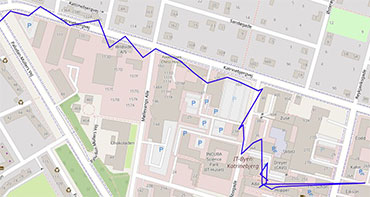
\includegraphics[width=\linewidth]{RouteWithOutFilter2.jpg}
    \caption{Without median filter (blue line)}
    \label{fig:route_without_filter}
\end{minipage}\hfill
\begin{minipage}{0.49\textwidth}
\centering
    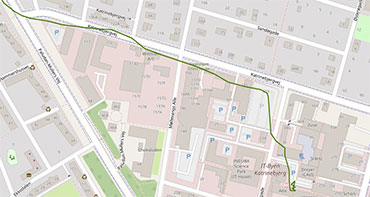
\includegraphics[width=\linewidth]{RouteWithFilter2.jpg}
    \caption{With median filter (green line)}
    \label{fig:route_with_filter}
\end{minipage}
\end{figure}

To get a better overview, both of the following maps are rotated. The DP compression is applied on figure \ref{fig:douglas_peucker_compression}. After applying the DP the routes is compressed to 20 location points, which is nearly a saving of 96\%. Figure \ref{fig:sliding_window} shows the route after applying Sliding window. For this prototype the code simulates how location points arrives periodically to be processed by the sliding window algorithm. The compression results in 304 location points, which is $50\%$ compression of the original route.

\begin{figure}[H]
\centering
\begin{minipage}{0.49\textwidth}
\centering
    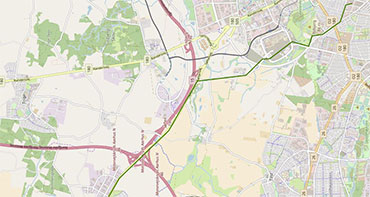
\includegraphics[width=\linewidth]{RouteDP2.jpg}
    \caption{Douglas Peucker compression (green line)}
    \label{fig:douglas_peucker_compression}
\end{minipage}\hfill
\begin{minipage}{0.49\textwidth}
\centering
    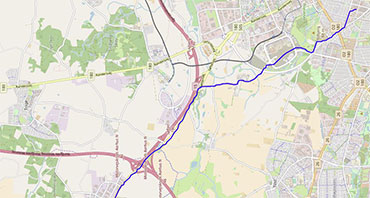
\includegraphics[width=\linewidth]{RouteSW2.jpg}
    \caption{Sliding window compression (blue line)}
    \label{fig:sliding_window}
\end{minipage}
\end{figure}

Since the core engine of BikeBus is build on a flexible architecture, it should be manageable to plug these algorithms into BikeBus. When pluggin compression algorithm into Bikebus more testing has to be done on how it affects the energy consumption.

Figure \ref{lst:sliding_window_code} is an implementation of the sliding window. Basically it follows the steps described in figure \ref{fig:sliding_window_algorithm}. 

\lstinputlisting[label={lst:sliding_window_code}, caption={Sliding window}, language={Python}]{Graphics/Images/SlidingWindow3.py}

To achieve the open window algorithm one only needs to change the point added to the approximated trajectory and the new anchor point. As described in figure \ref{fig:open_window_algorithm} the open window chooses the point with largest distance when the threshold is violated. Listing \ref{lst:open_window_code} shows a minor change in the loop which get the location point within the window with the largest error rate. The results for the open window implementation needs more investigation before any statement can be concluded. 
\lstinputlisting[label={lst:open_window_code}, caption={Open window}, language={Python}]{Graphics/Images/OpenWindow2.py}


\subsection{Distance calculation}
% Remember to reference to search - connect to search functionality

Searching routes is bounded to a distance calculator. By encapsulated the distance calculation, the search is robust to changes. The first implementation was the simple distance calculator which consist of a primitive euclidean distances calculation. Later when the Google API was integrated the Google distance matrix was implemented. By using a strategy pattern \cite{Baerbak10} it was uncomplicated to implement the new calculator without breaking existing functionality. 

\begin{figure}[H]
\centering
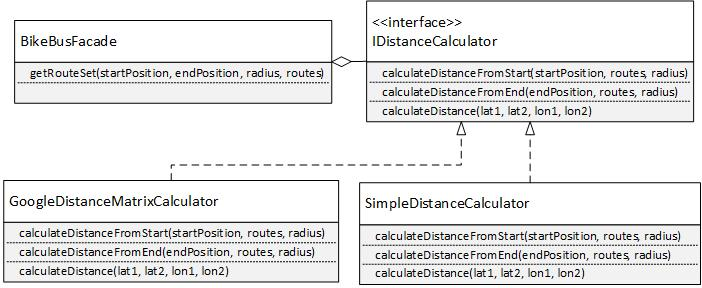
\includegraphics[scale=0.6]{Distance.jpg}
\caption{Module viewpoint of the strategy pattern of distance calculation}
\label{fig:module_view_distance_calculation}
\end{figure}

The search with Google distance matrix results in a minor latency compared with euldian computation.    

\subsection{Activity recognition and location}
\label{section:Activity_recognition_and_location}
As stated in section \ref{subsec:modifiability} the encapsulation tactic was chosen to achieve modifiability on replacing the sensor framework. The encapsulation is realized by coding to small interfaces and thereby achieving low coupling and high cohesion. Figure \ref{fig:activity_regonition_module_viewpoint} is a rough overview of the relations between the core classes gathering sensor data when biking.  
Notice that every class is encapsulated behind an interface. This also holds true for the activity recognition package seen in figure \ref{fig:Module_View_Sensor_Data}. It should be durable to hold the response measure by doing change by addition \cite{Baerbak10}.    

\begin{figure}[H]
\centering
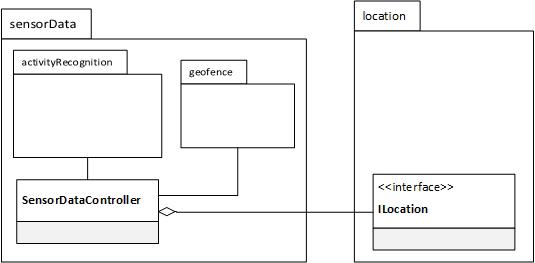
\includegraphics[scale=0.6]{ActivityRegonitionModuleViewpoint.png}
\caption{Module viewpoint of sensorData and location package}
\label{fig:activity_regonition_module_viewpoint}
\end{figure}

In section \ref{sec:continuous_sensing_Architecture} the flow of the components are explained which also addresses the energy efficiency tactic in section \ref{subsec:energy_efficiency}. Sensor selection is done by first visiting activity recognition before pulling location data.   

\subsection{Google services}
\label{section:google_services}
%Admir
Throughout BikeBus' development process Google services have been made use of. Below a list of Google services can be seen each service was implemented best practice according to the source and was incorporated into the interface and listener structure as mentioned in section \ref{sec:interfaces_and_listeners}. The interfaces and listeners for the below services can be seen in figure \ref{fig:interfaces}.\\

\noindent{The list contains eight services, each followed by a link explaining the implementation.}

\begin{itemize}
    \item Activity Recognition \cite{googleActivityRecognition}
    \item Distance Matrix Calculator \cite{googleDistanceMatrix}
    \item Firebase \cite{googleFirebase}
    \item Fused Location \cite{googleFusedLocation}
    \item Geocoder \cite{googleGeocoder}
    \item Geofence \cite{googleGeofencing}
    \item Login with Google \cite{googleActivityRecognition}
    \item Place Autocomplete \cite{googleAutocomplete}
\end{itemize}

\subsection{Data Layer implementation}
Following section will briefly illustrate how data is created, stored and read, in addition to what is mentioned as best practice in section \ref{section:google_services}. For this creating a route will be used as an example. 

In order to create a route a domain object of Route is necessary. Such object contains properties such as id, date, arrival time, departure time and several others as seen in "Routes.java" class under the "domain" package. This will allow "CreateActivity.java" to pass route related data to "BikeBusFacade.java", which is a common repository for data, and implements the IFacade interface. From the data facade, the "IStorage.java" interface is also made use of. The "IStorage.java" has two listeners for when retrieving data "OnGetRoutesListener" and "OnGetUsersListener". Each of these interfaces can be seen in the appendix \ref{app:interfaces}.

Once the data for creating a route has been passed all the way to the "saveRoute" method it is now possible to save the route to the Firebase database. As seen in listing \ref{code:saveRoute} a routes cloud endpoint is referenced, which points to the "routes" JSON object, and an UUID is set for the route, as seen previously in section \ref{sec:data_layer_design}.

\begin{lstlisting}[frame=single, language=Java, label={code:saveRoute}, caption={Save route to database}]
public String saveRoute(Route route) {
    routesCloudEndpoint.child(route.getId()).setValue(route);
    return route.getId();
}
\end{lstlisting}

To read routes from the database the "getRoute" method is made use of as seen in listing \ref{code:readRoute}. As seen in the code the "onDataChange" event method iterates through all the routes in the database using a "dataSnapshot" object, which contains the data from the "routes" database location in Firebase. The value from the for loop is parsed to the "Route.java" class if UUID equals the specified "id" parametre. 

\begin{lstlisting}[frame=single, language=Java, label={code:readRoute}, caption={Read routes from database}]
public void getRoute(final String id, final OnGetRoutesListener listener) {
    listener.onStart();
    routesCloudEndpoint.addValueEventListener(new ValueEventListener() {
        @Override
        public void onDataChange(DataSnapshot dataSnapshot) {
            List<Route> routes = new ArrayList<Route>();
            for (DataSnapshot userSnapshot : dataSnapshot.getChildren()) {
                if (userSnapshot.getKey().equals(id)) {
                    Route route = (Route)userSnapshot.getValue(Route.class);
                    routes.add(route);
                    break;
                }
            }
            listener.onSuccess(routes);
        }
        @Override
        public void onCancelled(DatabaseError databaseError) {
            Log.d("detailedResultsActivity", databaseError.getMessage());
            listener.onFailed(databaseError.getCode() + ": "+ databaseError.getMessage());
        }
    });
}
\end{lstlisting}


Alternatively, it is also possible to simply create a "DataSnapshot" object at a specific route item, this would be ideal should the database grow exponentially, as it would not require one to iterate through all of the route objects in the database.



%Admir

%TODO:
% - Take either "getUser" or "getRoute" methods and describe the "onDataChange" method
%    - for loop: parse value to Route.class if UUID equals parameter
%    - call listener.onSuccess to return async results
% - Describe other ways to do this
%    - create datasnapshot at a specific route/user item given UUID instead of retrieving all routes/users and iterating through everything
%    - Pros: faster
%    - Cons: When firebase class is initialised we end up creating quite many datasnapshots (is that a good idea?)


% Interfaces can be refered to in appendex \ref{fig:interface}. Remember to point out the specific interface your want to explain








